\documentclass[11pt]{report}

\usepackage{fullpage, url, graphicx, geometry, setspace}
\newgeometry{left=0.8in, right=0.8in, bottom=4cm, top=0.9in}
\onehalfspacing

\begin{document}

\thispagestyle{empty}

	\begin{center}
		
\includegraphics[scale = 1.9]{./images/WarwickCrest.pdf}
	\end{center}
	\vspace{8mm}
	\begin{center}
		\bf {\Large Data mining Twitter for analysis and user comparisons}
	\end{center}
	\vspace{5mm}
	\begin{center}
		\bf {\Large CS310 - Third Year Project Final Report}
	\end{center}
	\vspace{20mm}
	\begin{center}
		{\bf Caroline Player\\
		1112108}
	\end{center}
	\vspace{20mm}
	\begin{center}
		{\bf Department of Computer Science\\University of Warwick\\\vspace{6mm}
		2013-2014}
	\end{center}

\pagenumbering{roman}

\tableofcontents

\listoffigures
\newpage

\setcounter{page}{1}
\pagenumbering{arabic}


\chapter{Introduction}
The project documented in this report is about extracting meaning from data made available by the social media Twitter. This report will demonstrate the research which lead to what was ultimately built and the system requirements that are justified by the research, followed by how the project was designed, implemented and managed, an evaluation of the success of the project and finally a conclusion. This chapter outlines the aims and motivations of the project.
%Learn the difference of who and whom
\section{Motivation}
A new technology, still in it's infancy, is being developed to gather meaning behind data on the internet. This technology is called the Semantic Web. Currently, one of the biggest projects involved in the Semantic Web is DBPedia, an ontology of the entirity of Wikipedia. By exctracting meaning from such large data sets, a computer can tell you what an article is talking about without it explicitly being told. 
%Give this a little more explanation
Another popular research area is sentiment analysis of social media such as Twitter. The aim of which is to understand what users of the social media are talking about at a point in time, or feelings towards a specific topic, and then exploiting that knowledge for individual purposes.
These technologies are advancements in artificial intelligence in computing, and they can be further developed to optimise the information we can gain from this data and how it is used. 

\section{Project Aims}
The aim of this project is to develop software that can take available data from Twitter and produce a visualisation that displays relevant topics talked about on Twitter and for each user what that topic means to them. The outcome of this project is a unique representation of Twitter users.
This sentiment anlysis aims to dynamically understand what is being talked about on Twitter and to who it is meaningful.


\chapter{Research}
This chapter documents the research that was undertaken for this project. The research shows similar and related work that was used to invistigate the area of unbiased sampling of directed and undirected graphs, sentiment analysis and speech. 
\section{Existing Systems}
\subsection{Alchemy API}

\section{WordNet}
A synset is a set of synonyms. 
WordNet can be interpreted and used as a lexical ontology [Wikipedia]. However such an ontology should be corrected before use since it contains hundreds of basic semantic inconsistencies such as 
i) the existence of common specializations for exclusive catgories and 
ii) redundancies in the specialization hierarchy.
Furthermore, transformation of WordNet to an ontologyshould involve 
i) distinguishing the specialization relations subtypeOf and instanceOf relations, an
ii) associating intuitive unique identifiers to each category

Main relation among words in WordNet is synonym (as between the words shut and close, or car and automobile). These get grouped into unordered set - synsets. WordNet has 117000 synsets

A hyperonym/hypernym is the super-subordinate relation. It links a word such as furniture, to bed like this \{furniture, peice\_of\_furniture\}. This is transitive. If Armchair is a kind of chair, and if a chair is a kind of furniture, then armchair is a kind of furniture. Instances are always leaf nodes in their hierarchies. 

Meronymy, the part-whole relation holds between sysets like {chair} and {back, backrest}, \{seat\} and \{leg\}. Parts are inherited from their superordinates. If a chair has legs, an armchair has legs. They don't go upwards. E.g chair and counter are both furniture, a chair has legs, but furniture doesn't inherit taht upwards because that would mean counter has to inherit it and it doesn't.

Verb synsets are arranged into hierarchies as well. Verbs towards the bottom of the trees express increasingly specific manners characterizing an event, as in {communicate}-{talk}-{whisper}. The specific manner expressed depends on teh semantic field it's in, in this case, volume. Others are speed: {move}-{jog}-{run}, or intensity of emotion: {like-love-idiolize}.

Part of speech (POS). Wordnet cosists of four sub-nets, one each for nouns, verbs, adjectives and adverbs, with few cross-POS pointers. Cross-POS relations include the morphosemantic links that hold among semantically similar words sharing a stem with the same maeaning: observe(verb), observant(adj) observation, observatory (nouns). 


\subsection{Classes}
Word: 
getSynset

\section{Stanford Parser}
%Go through the manual and find where it points out a flaw. Such as not developed thoroughly

\section{Sentiment Analysers}
Most sentiment analysers available are aimed at picking at a speicific topic and assessing the feelings towards it. 
%My project aims to find categories in teh text. Later assessing who enjoys it and whetehr they get a 1 or a 0 for the category

\section{Literature Review}
\subsection{Recognizing Contextual Polarity in Phrase-Level Sentiment Analysis}
%Basically verbatim from paper. Rewrite. 
This paper looks at how phrase level sentiment analysis can determine positive and negative expressions~\cite{phraselevelsentimentanalysis}. 
We can pick out keywords in a phrase and look at their {\bf prior polarity}. This is their polarity before we put it in context. This paper discusses new experiments in automatically distinguishing prior and contextual polarity: They use a two step process that uses machine learning and a variety of features. 
\begin{itemize}
\item First step classifies each phrase containing a clue as neutral or polar.
\item Second step takes all phrases marked in step one as polar and disambiguates their contextual polarity.
\end{itemize}
The system can now automatically identify contextual polarity for a large subset of sentiment expressions.
\subsection{Combining strengths, emotions and polarities for boosting Twitter sentiment anlaysis}
This paper proposes an approach for boosting Twitter sentiment classification using different sentiment dimensions as meta-level features~\cite{combiningstrengthsemotionspolarities}. They combine aspects such as opinion strength, emotion and polarity indicators, generated by existing sentiment analysis methods and resources. The combination provides significant improvement in Twitter sentiment classification tasks such as polarity and subjectivity. 

Emoticons can introduce noise~\cite{combiningstrengthsemotionspolarities}.

\section{Tools}
\subsection{Stanford Natural Language Parser}
The parser tokenises the text and then tags each token with what it means gramatically i.e a verb, noun, adverb etc. Builds a parse tree for it. 

\chapter{System Requirements}
\section{Functional Requirements}


\section{Non-functional Requirements}


\chapter{System Design}
\section{System Overview}
Here is an image 
\begin{center}
		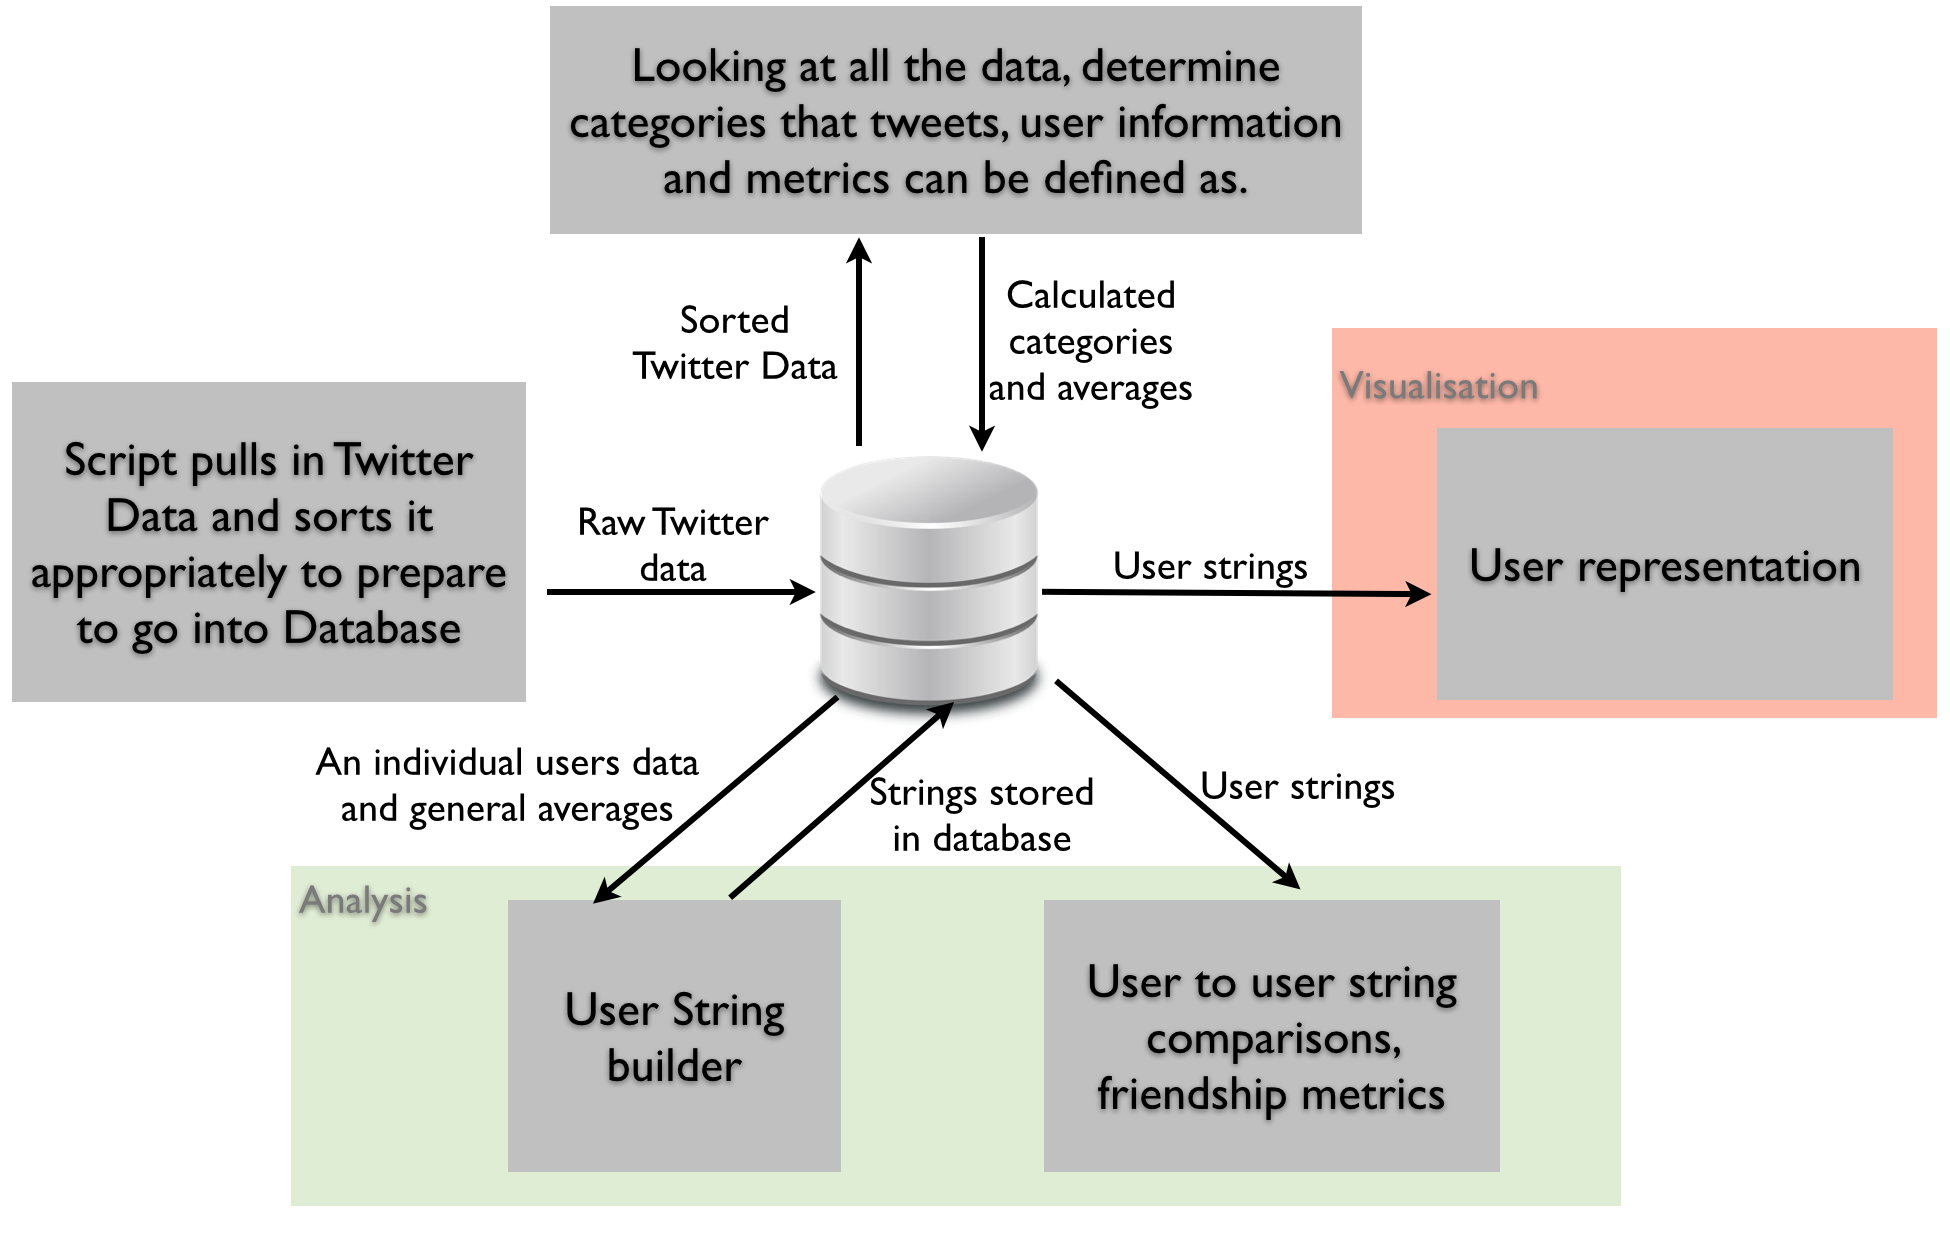
\includegraphics[scale = 0.55]{./images/architecture.png}
\end{center}
\section{Data Collection}
The first engine in the system is the data collection. Open source data sets are limited and not necessarily contianing relevant data, as well as possibly being biased towards certain topics, users or geographical locations, the need to produce a system which colleted data more relevant to this project was developed. 

\subsection{Database Design}
%Put schema in appendix!!!!
The idea of the Semantic Web is to give meaning to data, and in the case of Twitter this does not just mean the text in a users tweets. To understand more about a user, we can exploit information on Twitter:
\begin{itemize}
\item {\bf Tweets} - useful after having undergone analysis to extract meaning on interests and sentiment towards them. 
\item {\bf Following} - the types of people a user follows will indicate what they are interested in reading about
\item {\bf Followed By} - this is an indication of what they often tweet about. What is important to them that they feell should be expressed
\item {\bf Numerical Data} - such as how many friends and followers a user has. If very few they might be a Twitter sheep. 
\item {\bf Favourites and Retweets} - Giving stronger sentiment to the favourited tweets because they were found particularly important by the user. Or if a user has tweeted a particularly popular tweet then maybe they are more of an authority on this area. 
\item {\bf Hashtags} - used for emphasis on the object(?) of the conversation. Might give the topic more relavance to the user.
\end{itemize}
Hundreads of thousands of tweets are stored in the database and so an efficient schema needed to be designed in order to optimise space. This was done by only storing the text of the tweet once with details about it, such as how many times it was retweeted or favourited, by who it was made and it's ID. Then any retweet could simply reference the tweet ID in a separate table.
The database needed to be normalised for references. Tweets split into the tweet and it's details. Then a separate table for the users and referencing which tweets they said from the tweet table. 

\subsection{Unbiased Sampling of Twitter}
The graph that was being sampled consisted of nodes which were users and edges between them which indicated one relationship of either following or being followed by. When travelling between nodes it therefore makes the more popular users of Twitter much more likely to be visited repeatedly. It is important to note that if a user is popular and we would like to understand them better to see why they are so popular as this is useful information on what other users are interested in, but not in excess. Visiting many other users that have limited connections is also important. Therefore we can apply what is called the Metropolis-Hastings Random Walk algorithm to try and collect an unbiased sample of Twitter, where we are avoiding the bias of frequently visiting popular Twitter users.

\section{Analysis}
blah

\chapter{Implementation}
\section{Data Collection}
\subsection{Tools}
The tools used for this were the Twitter API which provides HTTP requests that return JSON objects.
\subsection{Joshua}
When a certain amount of data has been collected from Twitter, a waiting time must be obeyed before you can continue collecting more data. The amount of data that can be collected can be seen in appendix (DO AN APPENDIX ON THE TWITTER API)

\section{Analysis}


\subsection{Twitter Content}
Before users could be given a string which represents whether or not they are interested in certain categories, the categories need to be defined. Determining the categories could not be hardcoded because this would not encapsulate all the topics discussed on Twitter, and lead to a misrepresentation about what is presented. Therefore, what was needed was a system to analyse the text of tweets, and dynamically create the categories, creating data driven results. The following section discusses how the design discussed in Chapter~\ref{chap:design}, for categorising the text in tweets was implemented.
\subsubsection{Lexical Parsing}
The standford parser takes in any amount of text, and tokenises the words. Relationships between words are formed and a tree of the sentence structure can be produced. 
\subsubsection{Categorising content}
WordNet's database of words is limited, and therefore, before a word found in a tweet can be used for categorising, we have to clean it of punctuation, but most importantly, the stem of the word needs to be used. For example, `Flowers' would raise an exception if searched for in the WordNet dictionary, because it is a plural. So all words being used in analysis are first sent to a method to have the stem of the word found, and the stem is returned and used. This is still subject to errors as often the stemmer provided by the WordNet API returns latin words whose definitions are not stored in it's dictionary. Therefore sanity checks are in place to iterate through all the possible stems of a word and return the first word which applicable that has a definition. 
WordNet hypernym relation.
\subsubsection{Tools}
%not necessarily keeping the strcture of this chapter like this, however this is a way of keeping note of the tools used so far in development
\begin{itemize}
\item {\bf Alchemy API} Has restrictions of 1,000 calls a day and supports a maximum of 5 concurrent requests.API Notes:

Calls to TextGetRankedKeywords should be made using HTTP POST.
HTTP POST calls should include the Content-Type header: application/x-www-form-urlencoded
Posted text documents can be a maximum of 150 kilobytes. Larger documents will result in a "content-exceeds-size-limit" error response.
Language detection is performed on the retrieved document before attempting keyword extraction. A minimum of 15 characters of text must exist within the requested HTTP document to perform language detection.
Documents containing less than 15 characters of text are assumed to be English-language content.
Keyword extraction is currently supported for all languages listed on the language support page. Other non-supported language submissions will be rejected and an error response returned.
Enabling keyword-level sentiment analysis results in one additional transaction utilized against your daily API limit. Keyword-level sentiment analysis is currently provided for both English and German-language content.
\end{itemize}

\subsection{User Sentiment Analysis}
%This discusses whether an individual user gets a 1 or 0 for the categories determined in the "Twitter Content section"

\chapter{Testing}

\chapter{Project Management}
\section{Data Management}
Database snapshots

\chapter{Evaluation}

\chapter{Conclusion}



\bibliography{bibliography}
\bibliographystyle{plain}

\end{document}

